% !TeX spellcheck = en_US
\documentclass[aspectratio=1610]{beamer}
\usetheme{Madrid}
\setbeamercovered{transparent}
\setbeamertemplate{navigation symbols}{}
\setbeamertemplate{itemize items}[circle]
\setbeamertemplate{enumerate items}[default]

\makeatletter
\define@key{beamerframe}{wide}[10pt]{%
	\def\beamer@cramped{\itemsep #1\topsep0.5pt\relax}}
\makeatother
	

\usepackage[english]{babel}
\usepackage[utf8]{inputenc}
\usepackage[T1]{fontenc}
\usepackage{array}
\usepackage{xcolor}
\usepackage{colortbl}
\usepackage{booktabs}

\title[Winter - Lecture 7] % (optional, use only with long paper titles)
{Intermediate Macroeconomics: Lecture  W7 (Ch. 18)}
\subtitle{ECON 311 -- Intermediate Macroeconomics}

\author{Muhebullah Karimzada}
\institute{School of Economics \\\ University of Northern British Columbia}
\date{Fall 2026}


% ---------- UNBC COLORS ----------
\usepackage{xcolor}
\definecolor{UNBCGreen}{RGB}{0,102,51}
\definecolor{UNBCDark}{RGB}{0,74,37}
\definecolor{UNBCGold}{RGB}{189,155,96}
\definecolor{SoftCream}{RGB}{249,247,242}
\definecolor{SoftGray}{RGB}{244,246,248}
\definecolor{AccentBlue}{RGB}{41,98,255}
\definecolor{AccentOrange}{RGB}{230,126,34}
\definecolor{AccentTeal}{RGB}{0,150,136}
\definecolor{AccentRed}{RGB}{192,57,43}
\setbeamercolor{normal text}{fg=black,bg=white}
\setbeamercolor{structure}{fg=UNBCDark}
\setbeamercolor{title}{fg=white,bg=UNBCDark}
\setbeamercolor{subtitle}{fg=UNBCGold}
\setbeamercolor{frametitle}{fg=white,bg=UNBCDark}
\setbeamercolor{block title}{fg=white,bg=UNBCDark}
\setbeamercolor{block body}{fg=black,bg=SoftGray}
\setbeamercolor{block title alerted}{fg=white,bg=AccentRed}
\setbeamercolor{block body alerted}{fg=black,bg=SoftGray}
\setbeamercolor{item}{fg=UNBCDark}
\setbeamercolor{section in toc}{fg=UNBCDark}
\setbeamercolor{alerted text}{fg=AccentRed}
\setbeamercolor{author in head/foot}{fg=white,bg=UNBCDark}
\setbeamercolor{date in head/foot}{fg=white,bg=UNBCDark}
% ---------- UNBC BRANDING ----------
\usepackage{graphicx}
\usepackage{lmodern}
\usepackage{tcolorbox}
\usepackage{tikz}
\usetikzlibrary{positioning,calc}
\setbeamertemplate{headline}{}
\setbeamertemplate{footline}{%
  \leavevmode%
  \hbox{%
  \begin{beamercolorbox}[wd=.78\paperwidth,ht=2.8ex,dp=1.2ex,leftskip=1em]{author in head/foot}%
  \color{white}\textbf{ECON 311} \hspace{0.5em} \textcolor{UNBCGold}{|} \hspace{0.5em} Intermediate Macroeconomics%
  \end{beamercolorbox}%
  \begin{beamercolorbox}[wd=.22\paperwidth,ht=2.8ex,dp=1.2ex,rightskip=1em plus1fil]{date in head/foot}%
  \color{white}\insertframenumber/\inserttotalframenumber%
  \end{beamercolorbox}}%
}

\newtcolorbox{mybox}[2][]{
  colback=#2!8,
  colframe=#2,
  boxrule=0.8pt,
  arc=2mm,
  left=2mm,right=2mm,top=1.5mm,bottom=1.5mm,
  #1
}

\newcommand{\topbanner}[1]{%
\begin{tikzpicture}[remember picture,overlay]
\fill[UNBCGold] ([yshift=-0.65cm]current page.north west) rectangle ([yshift=-0.48cm]current page.north east);
\node[anchor=north west,font=\small\bfseries,text=UNBCDark] at ([xshift=0.35cm,yshift=-0.78cm]current page.north west) {#1};
\end{tikzpicture}%
}
\begin{document}

\begin{frame}[plain]
  \titlepage
\end{frame}


\begin{frame}[wide]{What are You Going to Learn (Ch. 18)}
	\begin{itemize}
		\item Government spending, taxation, budget deficits, and the debt-GDP ratio nationally and globally
		\vspace{3mm}
		\item The government’s intertemporal budget constraint
		\vspace{3mm}
		\item The economic consequences of budget deficits
		\vspace{3mm}
		\item The fiscal problem of the twenty-first century: how to finance rising health expenditures
	\end{itemize}
\end{frame}

%\begin{frame}[wide]{Introduction}
%	\begin{itemize}
%		\item The government can finance expenditures by
%		\begin{itemize}
%			\item using tax revenue
%			\item printing money
%			\item borrowing
%		\end{itemize}
%		\item But the government’s budget must balance in present value
%		\begin{itemize}
%			\item The amount the government spends must equal the amount the government earns in terms of present value
%			\item Budget deficits today must be offset by budget surpluses in the future
%		\end{itemize}
%		\item The “fiscal problem of the twenty-first century” 
%		\begin{itemize}
%			\item If current policies remain unchanged, forecasts show the U.S. and many other countries' deficits and debt-to-GDP ratios will explode
%		\end{itemize}
%		
%	\end{itemize}
%\end{frame}

\begin{frame}[wide]{U.S. Government Spending and Revenue}
	\begin{itemize}
		\item In 2018, government spending in the United States was 
		\vspace{4mm}
		\begin{itemize}
			\item \$6.7 trillion
			\item 20.0 percent of GDP
			\item more than \$20,500 per person! 
		\end{itemize}
		\vspace{6mm}
		\item Tax revenues were 16.2 percent of GDP 
	\end{itemize}
\end{frame}

\begin{frame}[wide]{The U.S. Federal Government Budget, 2018}

	\begin{figure}
		\centering
		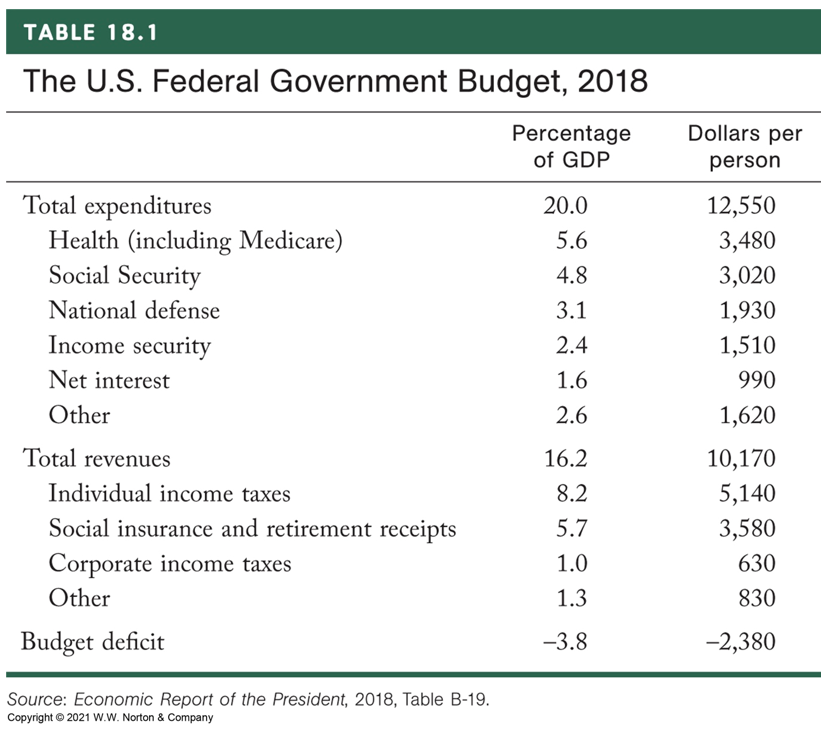
\includegraphics[width=0.6\linewidth]{Figures/fig_16_01}
	\end{figure}
	
\end{frame}



\begin{frame}[wide]{Government Spending and Revenue}
	\begin{itemize}
		\item The budget balance: The difference between tax revenues and spending
		\vspace{5mm}
		\item A budget surplus: Tax revenues > Spending
		\vspace{5mm}
		\item A budget deficit:	Tax revenues < Spending
%		\vspace{2mm}
%		\begin{itemize}
%			\item The government must borrow by selling bonds
%		\end{itemize}
		\vspace{5mm}
		\item A balanced budget: Tax revenues = Spending
	\end{itemize}
\end{frame}

\begin{frame}[wide]{Government Spending and Revenue}
	\begin{itemize}
		\item In 2018, there was a budget deficit equal to 3.8 percent of GDP (0.5 percent in Canada)
		\vspace{2mm}
		\begin{itemize}
			\item The government does not usually sell assets to finance the deficit
			\item Usually, the government borrows from lenders domestically and abroad
		\end{itemize}
		\vspace{5mm}
		\item When the government sells bonds, they use the money as a loan
%		\vspace{2mm}
%		\begin{itemize}
%			\item Suppose a 10-year bond issued in 2021 pays \$100 when it matures in 2031
%			\item In 2021, the investor may pay \$55 for this bond (and that amount is the loan to the government)
%			\item The remaining \$45 the government pays is the nominal interest
%		\end{itemize}
		\vspace{5mm}
		\item In 2018, the government issued more than \$750 billion in new bonds (>\$2,300 per person)
	\end{itemize}
\end{frame}


%\begin{frame}[wide]{Spending and Revenue over Time}
%	\begin{itemize}
%		\item After World War II, spending and tax revenues rose to about 18 percent of GDP
%		\vspace{2mm}
%		\begin{itemize}
%			\item The two were roughly the same fraction of the GDP
%		\end{itemize}
%		\vspace{4mm}
%		\item In 1970, systematic budget deficits began to emerge
%		\vspace{2mm}
%		\begin{itemize}
%			\item Deficits as a fraction of GDP peaked in 1983
%			\item There was a brief surplus in 1998, followed by another deficit in 2002
%		\end{itemize}
%		\vspace{4mm}
%		\item In 2009, the budget deficit was around 10 percent of GDP
%		\vspace{2mm}
%		\begin{itemize}
%			\item During the recession, tax revenues fell and government spending increased
%		\end{itemize}
%	\end{itemize}
%\end{frame}

\begin{frame}[wide]{U.S. Federal Government Revenue and Spending}
	\begin{figure}
		\centering
		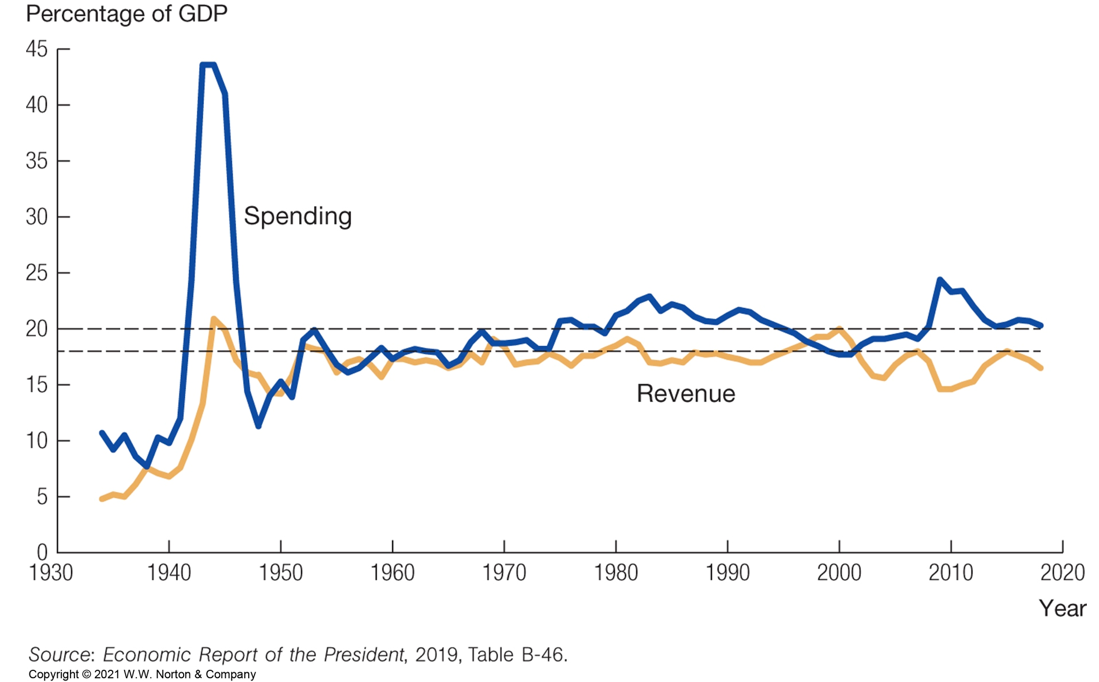
\includegraphics[width=0.7\linewidth]{Figures/fig_16_02}
	\end{figure}
	
\end{frame}

\begin{frame}[wide]{The Debt-GDP Ratio}
	\begin{itemize}
		\item Government debt: outstanding stock of bonds that have been issued in the past
		\vspace{2mm}
		\begin{itemize}
			\item It is like the capital accumulation function!
		\end{itemize}
		\vspace{4mm}
		\item In 2005, the debt-GDP ratio was just over 35 percent
		\vspace{4mm}
		\item In 2018, the debt-GDP ratio was nearly 80 percent, a huge increase
		\vspace{4mm}
		\item About half of the debt in recent years is owed to foreigners
	\end{itemize}
\end{frame}

%\begin{frame}[wide]{The Debt-GDP Ratio}
%	\begin{itemize}
%		\item The government itself also holds a large amount of bonds
%		\begin{itemize}
%			\item The Social Security trust fund that will be paid to future retirees held \$2.7 trillion in assets in 2014
%			\item One branch of government loaning to another has no affect on government “wealth.”
%			\begin{itemize}
%				\item The asset and debt created offset one another
%			\end{itemize}
%		\end{itemize}
%	\end{itemize}
%\end{frame}

\begin{frame}[wide]{Federal Debt and Deficits in the United States}
	\begin{figure}
		\centering
		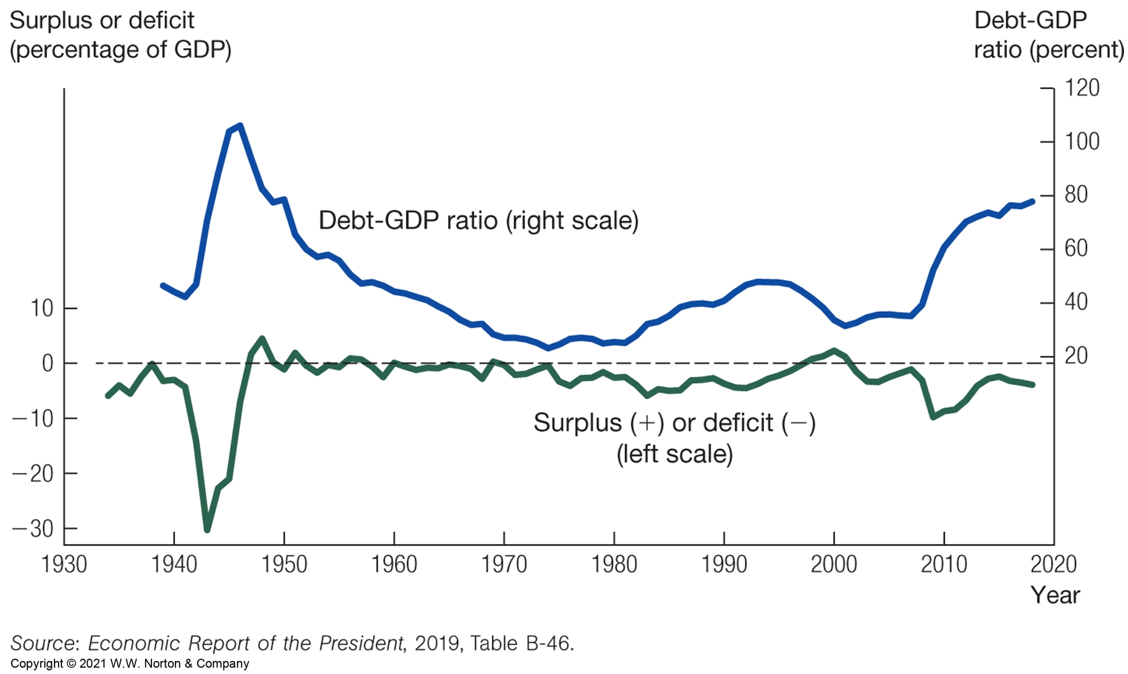
\includegraphics[width=0.7\linewidth]{Figures/fig_16_03}
	\end{figure}
\end{frame}

\begin{frame}[wide]{International Evidence on Spending and Debt}
	\begin{itemize}
		\item Among the richer OECD countries, the United States has a lower than average
		\vspace{2mm}
		\begin{itemize}
			\item government spending-to-GDP ratio
			\item debt-GDP ratio
		\end{itemize}
		\vspace{5mm}
		\item Norway is an exception among many rich countries
		\vspace{2mm}
		\begin{itemize}
			\item Negative debt-GDP ratio
			\item Norway benefits from large government-owned petroleum and natural gas reserves, which boost its revenues and lead to budget surpluses
			\item Knowing these revenues will be depleted, the Norwegian government saves these surpluses as assets in a Government Petroleum Fund to finance future government spending
		\end{itemize}
		
	\end{itemize}
\end{frame}

\begin{frame}[wide]{Government Spending around the World, 2017}
	\begin{figure}
		\centering
		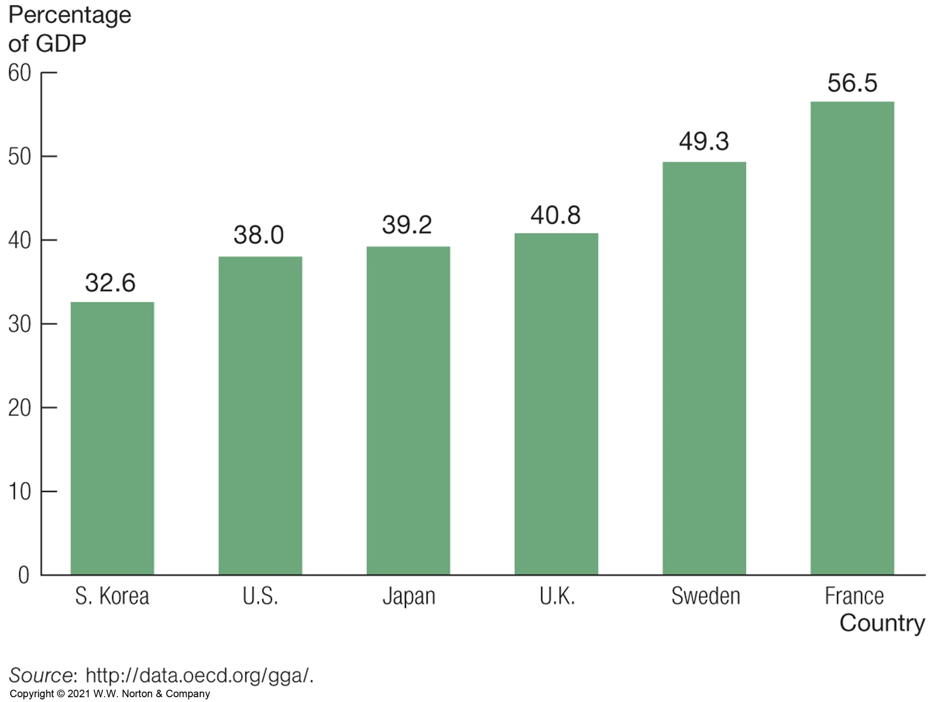
\includegraphics[width=0.6\linewidth]{Figures/fig_16_04}
	\end{figure}
	\vspace{5mm}
	Where would Canada fit?
\end{frame}

\begin{frame}[wide]{Debt-GDP Ratios around the World}
	\begin{itemize}
		\item In Japan, the ratio has risen sharply since 1995, from a low of about 20 percent to a high of more than 120 percent in 2018
	\end{itemize}
	\begin{figure}
		\centering
		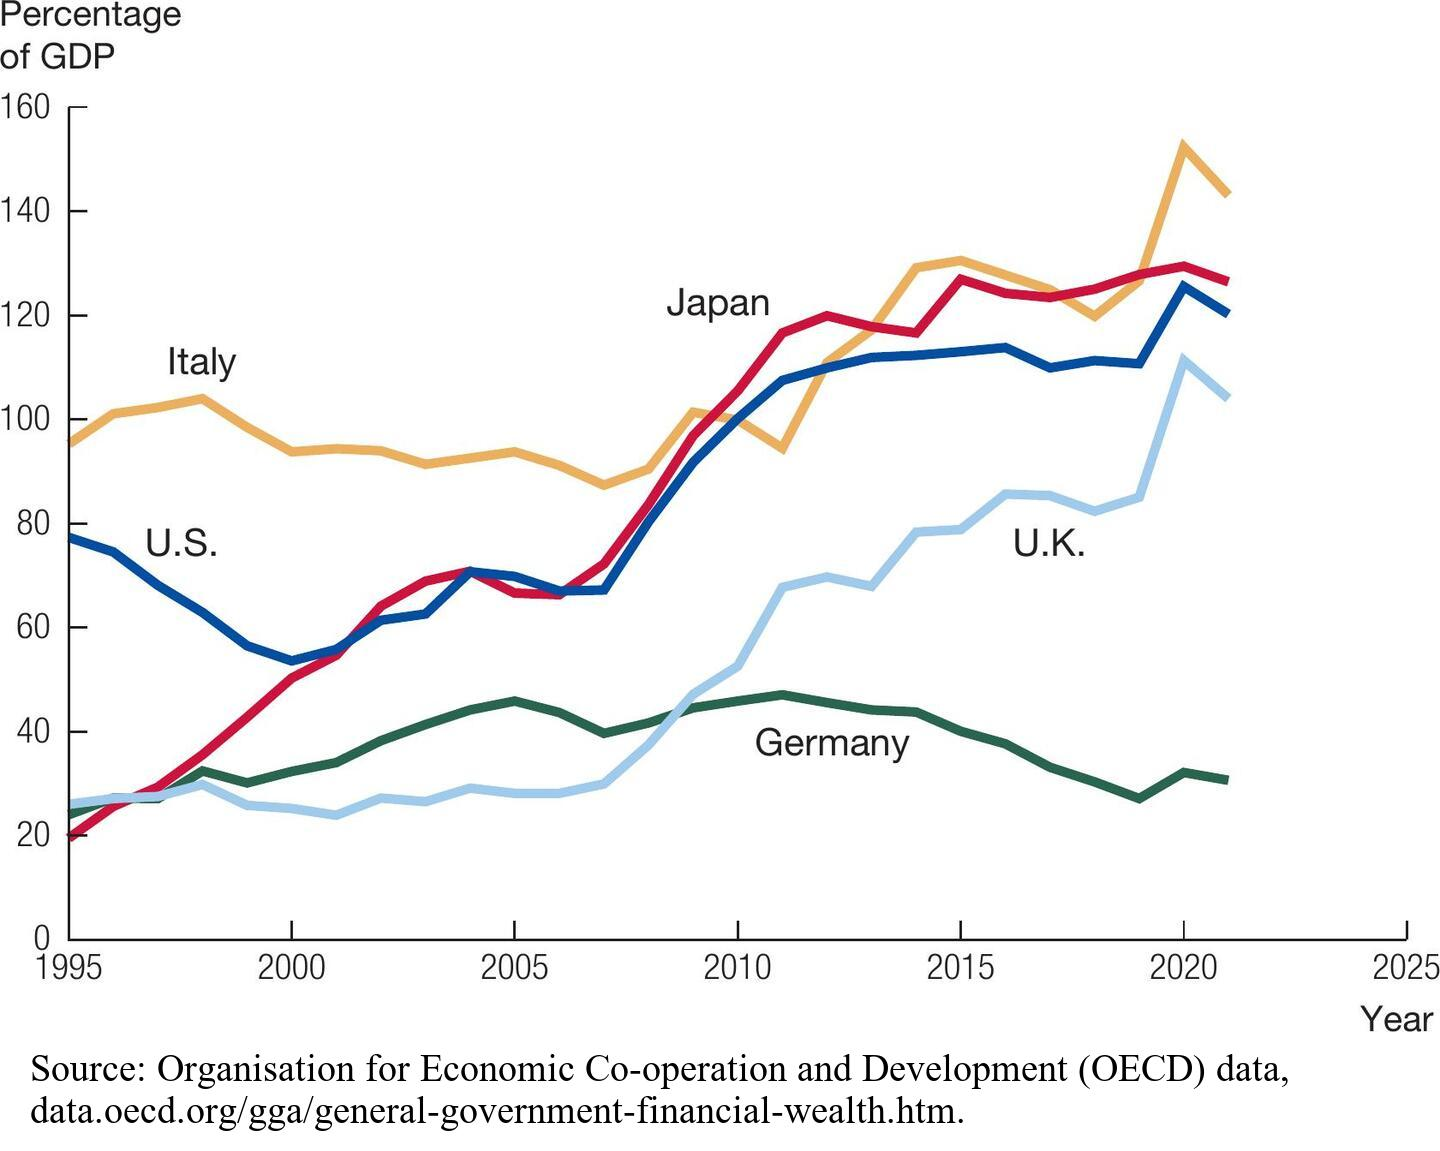
\includegraphics[width=0.6\linewidth]{Figures/MACRO6_FIG18.04}
	\end{figure}
	
\end{frame}

%\begin{frame}[wide]{Debt-GDP Ratios around the World}
%	\begin{itemize}
%		\item The net debt to GDP ratio varies a lot across country. But, higher number does not always mean a country is at risk. It depends on many country specific factor
%	\end{itemize}
%	\begin{figure}
%		\centering
%		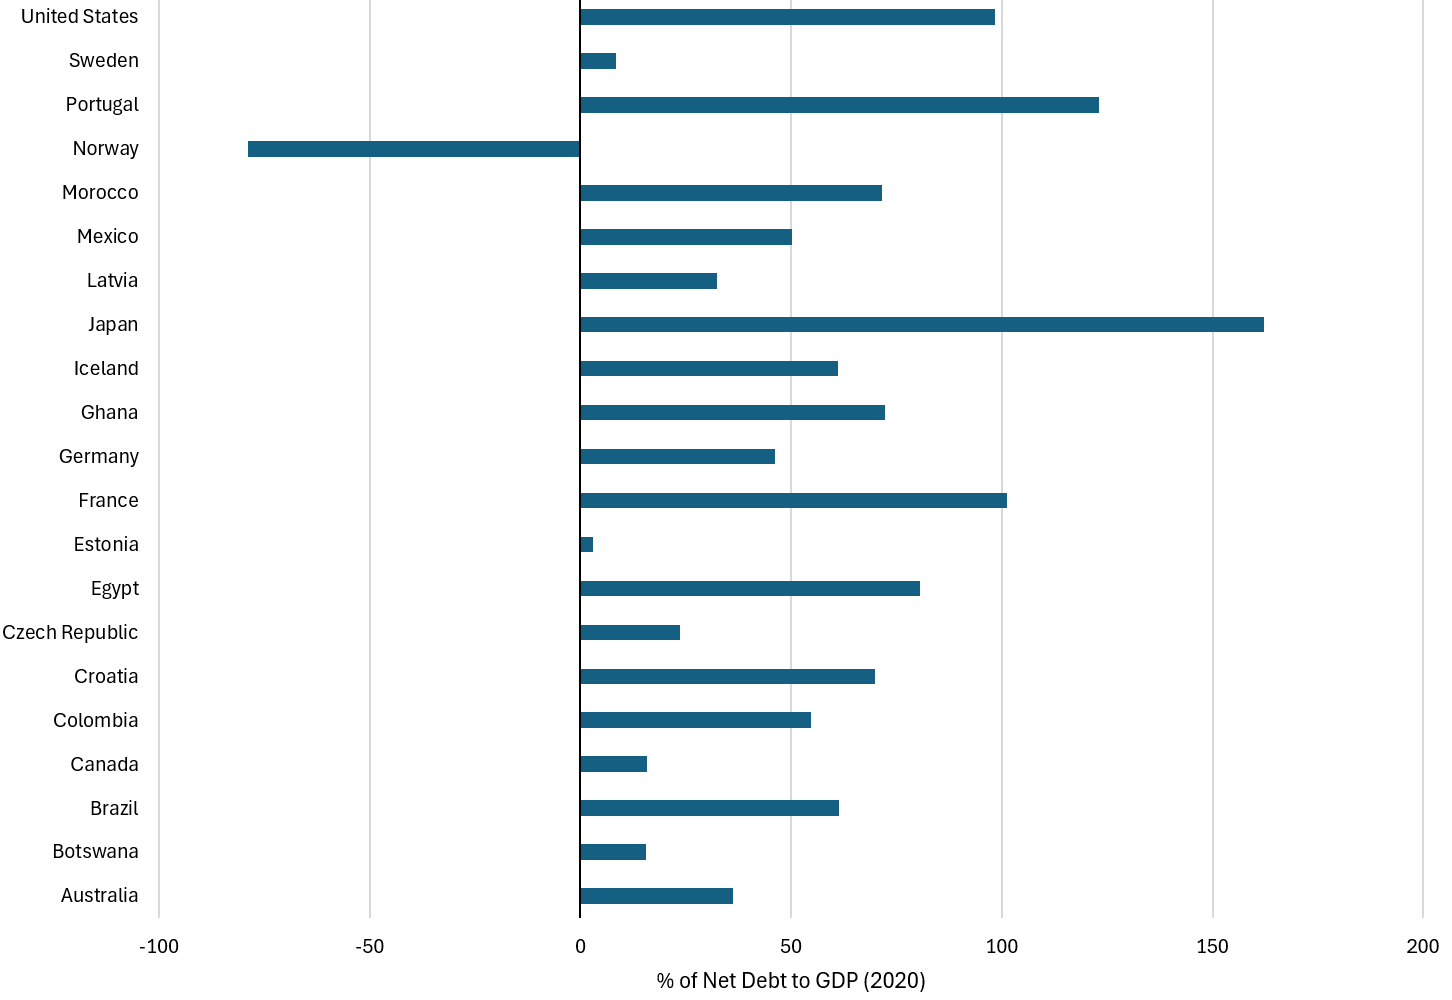
\includegraphics[width=0.7\linewidth]{Figures/fig_16_06}
%	\end{figure}
%	
%\end{frame}

\begin{frame}[wide]{Debt-GDP Ratios around the World}
	\begin{itemize}
		\item The Debt-GDP ratio comprises two components: Debt and GDP
		\vspace{8mm}
		\item If the GDP kept growing faster than debt, the debt-GDP ratio could decrease
		\vspace{8mm}
		\item When assessing the risk of a country defaulting, it's necessary to project the future growth of the country
		\vspace{2mm}
		\begin{itemize}
			\item Many factor could come into place as we learn in previous chapter
		\end{itemize}
	\end{itemize}

\end{frame}

\begin{frame}[wide]{The Government Budget Constraint}
	\begin{itemize}
		\item The flow version of the government budget constraint holds in each period
		\vspace{4mm}
		\item The sources of funds to the government must equal the uses of funds
		\vspace{1mm}
		\[G_t + Tr_t + (1+i)B_t = T_t + B_{t+1} + \Delta M_{t+1}\]
		\vspace{1mm}
		\item[] where $G_t$ is the gov't purchases, $Tr_t$ is the transfer payment, $i$ is the interest rate, $iB_t$ is the interest payments on debts, $T_t$ is the taxes, $\Delta B_{t+1}$ is the New Borrowing and $\Delta M_{t+1}$ is the change in money stock
		\vspace{4mm}
		\item $\Delta B_{t+1}$ and $\Delta M_{t+1}$ can be negative
	\end{itemize}
\end{frame}

\begin{frame}[wide]{The Government Budget Constraint}
	\begin{itemize}
		\item Assume for now, transfer payments are zero ($Tr_t = 0$)
		\[B_{t+1} = (1+i) B_t + G_t -T_t - \Delta M_{t+1}\]
		\vspace{2mm}
		\item LHS is the stock of debt at the start of next year 
		\vspace{4mm}
		\item RHS isthe Stock of debt this year, including the required interest payments plus the budget deficit and change in money supply
%		\vspace{4mm}
%		\item The primary deficit: $G_t - T_t$
%		\vspace{2mm}
%		\begin{itemize}
%			\item If the $G_t-T_t=0$, then the growth of $B$ is $g_B = \frac{B_{t+1}}{B_t} - 1 = i$
%		\end{itemize}
%		\item The total deficit: $G_t +iB_t -T_t$		
	\end{itemize}
\end{frame}
\begin{frame}[wide]{The Intertemporal Budget Constraint}
	\begin{itemize}
		\item Suppose an economy exists for only two periods
		\vspace{2mm}
		\begin{itemize}
			\item Period 1 could represent the country today, and period 2 could represent it in the future
		\end{itemize}
		\vspace{3mm}
		\item The budget constraint for period 1 is:
		\[B_2 = (1+i) B_1 +G_1 -T_1 - \Delta M_{2}\]
		\vspace{1mm}
		\item The budget constraint for period 2 is:
		\[B_3 = 0 = (1+i)B_2 +G_2 -T_2\]
		\vspace{1mm}
		\item $B_3=0$ is because No one is willing to lend as the economy live only for two periods (i.e., period 3 does not exist)
		\item Assume the money supply won't change between period 2 and 3
	\end{itemize}
\end{frame}

\begin{frame}[wide]{The Intertemporal Budget Constraint}
	\begin{itemize}
		\item Substitute the budget constraint for period 2 into period 1
		
		\[0 = (1+i)\left[(1+i) B_1 +G_1 -T_1 -\Delta M_{2} \right] +G_2 -T_2\]
		Divide both side by $(1+i)$
		\[0 = (1+i) B_1 +G_1 -T_1 -\Delta M_{2} +\frac{G_2 -T_2}{1+i}\]
		Rearrange:
		\[G_1 + \frac{G_2}{1+i} = T_1 + \frac{T_2}{1+i} - (1+i)B_1 + \Delta M_{2}\]
		\vspace{1mm}
		\item Present discounted value of spending (purchases) and initial debt must equal the present discounted value of tax revenues plus change in money supply
	\end{itemize}
\end{frame}

\begin{frame}[wide]{The Intertemporal Budget Constraint}
	\begin{itemize}
%		\item There is another way to interpret the equation
%		
%		\[T_1 - G_1 + \frac{T_2 - G_2}{1+i} = (1+i)B_1\]
%		
		\item The government’s budget must balance—not period by period, but rather in a PDV sense
		\vspace{3mm}
		\item The government must have surpluses in the future (today) to pay off deficits today  (future)
		\vspace{3mm}
		\item The implication is that the government must increase taxes at some point!
		\vspace{3mm}
		\item The logic of the intertemporal budget constraint applies for any number of time periods
	\end{itemize}
\end{frame}

\begin{frame}[wide]{How Much Can the Government Borrow?}
	\begin{itemize}
		\item The amount the government can borrow is limited by:
		\vspace{2mm}
		\begin{itemize}
			\item The amount it can credibly be expected to pay back
			\item Partly on how large the economy’s GDP is
		\end{itemize}
		\vspace{4mm}
		\item Recall that Debt-GDP ratio has two components	: Debt and GDP
		\vspace{2mm}
		\begin{itemize}
			\item If GDP grows faster than the stock of debt, this is not an issue
		\end{itemize}
		\vspace{4mm}
		\item When considering economic consequences of deficits and debts, we must consider
		\vspace{2mm}
		\begin{itemize}
			\item Economic growth
			\item The possibility of high inflation or default
			\item Intergenerational equity
			%\item The extent to which deficits crowd out investment
		\end{itemize}
		
		
	\end{itemize}
\end{frame}

\begin{frame}[wide]{High Inflation and Default}
	\begin{itemize}
		\item If the debt-GDP ratio becomes too high:
		\vspace{2mm}
		\begin{itemize}
			\item Lenders worry about the ability of the government to repay
			\item Investors demand higher interest rates
			\item This will itself prevent government borrowing from growing too large -- the government have to size down or turn to other sources (e.g., printing money)
		\end{itemize} 
		\vspace{4mm}
		\item If lenders stop lending (or at low enough interest rate):
		\vspace{2mm}
		\begin{itemize}
			\item The government may print more money to satisfy the budget
			\item This generates inflation
		\end{itemize}
	\end{itemize}
\end{frame}

\begin{frame}[wide]{High Inflation and Default}
	\begin{itemize}
		\item Default: Government cannot repay certain debts fully (or at less than face value)
		\vspace{6mm}
		\item This happened in a number of countries:
		\begin{itemize}
			\item Latin America during the early 1980s
			\item Russia in 1998
			\item Argentina in 2002 
			\item The euro crisis of recent years, which has already seen Greece “restructure” its debt
		\end{itemize}
	\end{itemize}
\end{frame}

%\begin{frame}[wide]{High Inflation and Default}
%	\begin{itemize}
%		\item In practice, the level of debt-GDP ratio that triggers a default varies across economy based on 
%		\begin{itemize}
%			\item Historical experience
%			\item Growth prospects
%			\item The credibility of the government and central bank
%		\end{itemize}
%	\end{itemize}
%\end{frame}

\begin{frame}[wide]{Generational Accounting}
	\begin{itemize}
		\item When the government borrows, the beneficiaries of borrowing may not be the same people who repay the debt
		\vspace{5mm}
		\item Example: World War II
		\vspace{2mm}
		\begin{itemize}
			\item The generation that fought the war made large sacrifices
			\item Future generations benefited from the victory
			\item Future generations paid for the war
		\end{itemize}
		\vspace{5mm}
		\item Generational accounting: 	Calculates the extent to which current policies pass on tax burdens to future generations
		
	\end{itemize}
\end{frame}

\begin{frame}[wide]{Generational Accounting}
	\begin{itemize}
		\item A study by Auerbach and Kotlikoff shows
		\vspace{2mm}
		\begin{itemize}
			\item Generations born in the 1980s and early 1990s would pay a lifetime tax rate of about 34 percent of their income
			\item All future generations would have to pay a lifetime tax rate of 71 percent
			\item High and rising debt-GDP ratios imply higher tax rates on future generations
		\end{itemize}
		\vspace{5mm}
		\item Achieving equalized lifetime tax rates across generations would require a significant change in current fiscal policy (e.g., tax rate based on age?)
		\vspace{5mm}
		\item Another debate is that 
		\vspace{2mm}
		\begin{itemize}
			\item Current would benefit from all those borrowings
			\item Future generations are likely to be richer, in part because of the investments in capital, education, and research done by current generation (through borrowing)
		\end{itemize}
	\end{itemize}
\end{frame}

%\begin{frame}[wide]{Deficits and Investment}
%	\begin{itemize}
%		\item The national income identity: 	Investment equals total saving
%		\[Y-C-G+(IM-EX) = I\]
%		\item Add and subtract tax revenues from the left side of the equation:
%		\[(Y-C-T)+(T-G)+(IM-EX) = I\]
%		\item There are three ways private investment can be financed:
%		\begin{itemize}
%			\item Saving from the private sector (Y - T – C) 
%			\item Saving by the government (T – G)
%			\item Saving by foreigners (IM-EX)
%		\end{itemize}
%		\item Crowding out: budget deficits may soak up saving in the economy and crowd out investment
%	\end{itemize}
%\end{frame}
%
%
%\begin{frame}[wide]{Deficits and Investment}
%	\begin{itemize}
%		\item Ricardian equivalence implies:
%		\begin{itemize}
%			\item Holding the present value of government spending constant, the timing of taxes does not affect consumption
%			\item Budget deficits need not crowd out investment
%			\item Instead, they will be offset exactly by higher private saving as individuals save to pay the future taxes implied by current budget deficits
%		\end{itemize}
%		\item Economists still debate the extent to which budget deficits crowd out investment
%	\end{itemize}
%\end{frame}

%\begin{frame}[wide]{U.S. Investment and the Budget Deficit}
%	\begin{itemize}
%		\item The investment rate in this same period has not really declined, despite the emergence of relatively large budget deficits since the 1980s
%		\item But a large rise in government saving was accompanied by a rise in the investment share
%	\end{itemize}
%	\begin{figure}
%		\centering
%		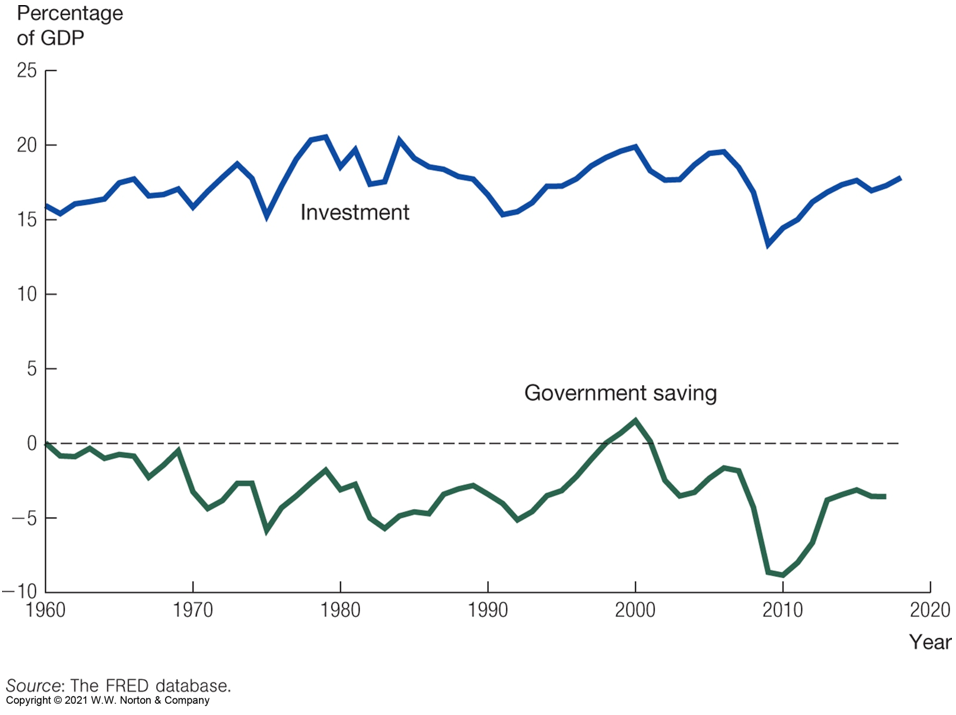
\includegraphics[width=0.5\linewidth]{Figures/fig_16_07}
%	\end{figure}
%	
%\end{frame}



\begin{frame}[wide]{The Fiscal Problem of the Twenty-First Century}
	\begin{itemize}
		\item In the coming decades, with current policies in place, according to a report from CBO, it is likely that by 2075:
		\vspace{4mm}
		\begin{itemize}
			\item Government spending will rise to 40 percent of GDP 
			\vspace{2mm}
			\item Annual budget deficits could reach 20 percent of GDP 
		\end{itemize}
		\vspace{5mm}
		\item Our current policies are unsustainable
	\end{itemize}
\end{frame}

\begin{frame}[wide]{The Problem}
	It is expected that the expenditure healthcare as a fraction of GDP will increase over time, because:
	\vspace{3mm}
	\begin{itemize}
		\item Increased generosity of entitlement programs
		\vspace{4mm}
		\item More people qualify:
		\vspace{2mm}
		\begin{itemize}
			\item In 1940, there were 8.6 people of working age for every person above 65
			\item In 2000, there were 4.7 people of working age for every person over 65
		\end{itemize}
		\vspace{4mm}
		\item Rise in health care expenditures (Medicare/Medicaid)
		\vspace{2mm}
		\begin{itemize}
			\item Health care costs per capita will grow at a rate of 1 percentage point faster than the rate of GDP growth
			\item 7.6 percent of GDP in 2000 to 13.9 percent in 2030 and 
			then to 21.1 percent by 2075
		\end{itemize}
	\end{itemize}
\end{frame}


\begin{frame}[wide]{U.S. Federal Spending and Revenues, 1950–2075}
	\begin{itemize}
		\item Health and retirement spending alone will exceed the percentage of GDP collected in taxes (assuming current policies)
	\end{itemize}
	\begin{figure}
		\centering
		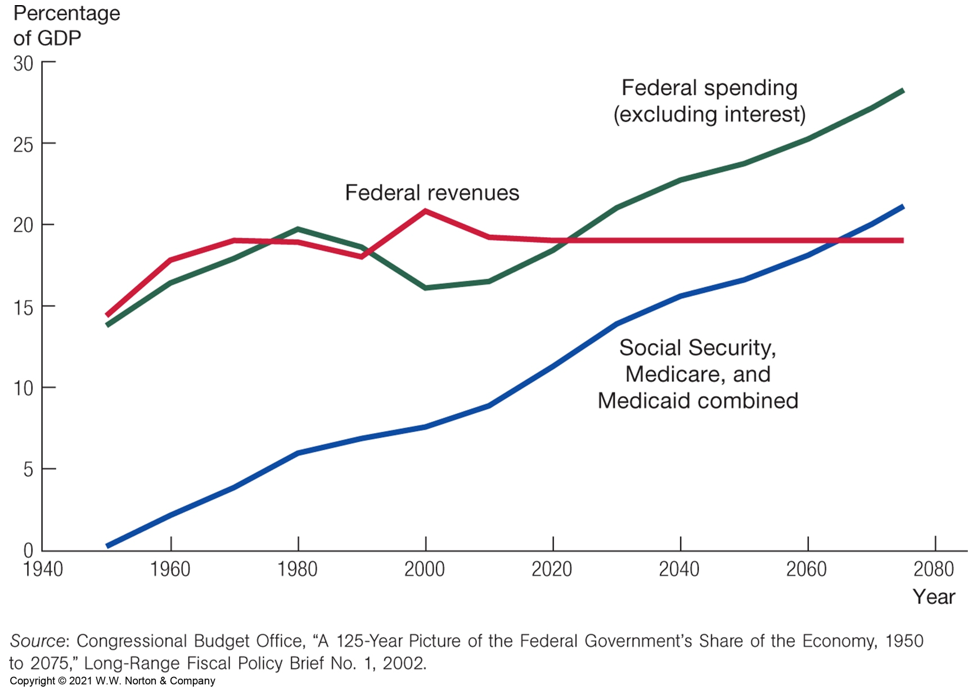
\includegraphics[width=0.6\linewidth]{Figures/fig_16_08}
	\end{figure}
	
\end{frame}

\begin{frame}[wide]{Components of Federal Spending, 1950–2075}
	\begin{itemize}
		\item The main culprit behind the rise in federal spending is health care then social security
	\end{itemize}
	\begin{figure}
		\centering
		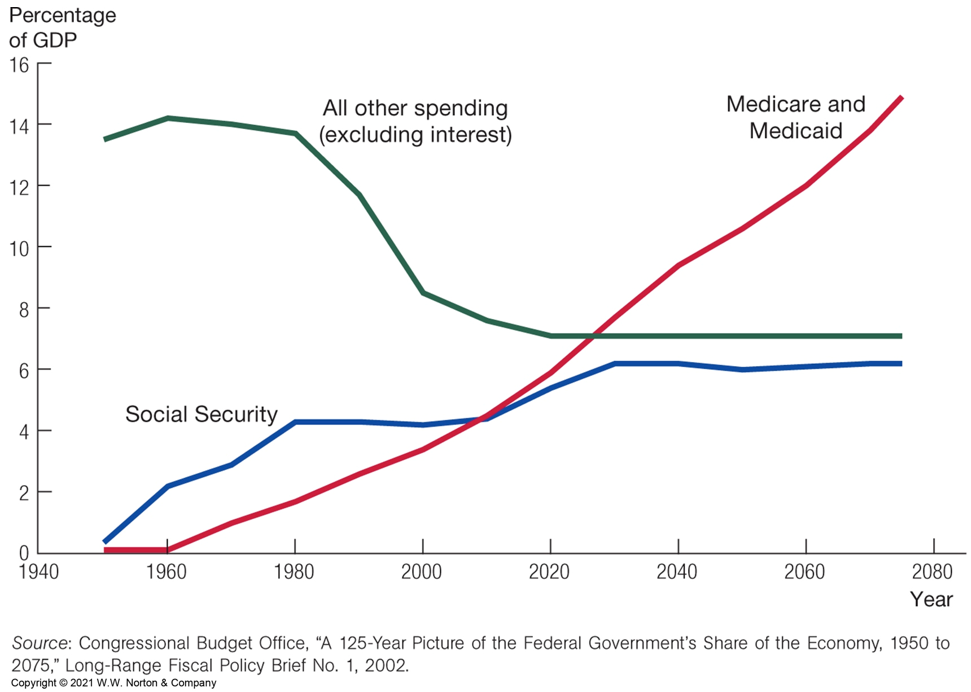
\includegraphics[width=0.7\linewidth]{Figures/fig_16_09}
	\end{figure}
	
\end{frame}

\begin{frame}[wide]{Financing the Social Security Program}
	\begin{itemize}
		\item Social security ensures retirees will be able to maintain standards of living
		\vspace{2mm}
		\begin{itemize}
			\item The current tax rate on wage income is 12.4 percent (half paid by employers)
			\item In Canada, the rate is around 11.9 percent
		\end{itemize}
		\vspace{4mm}
		\item Financed by an employment tax on wage income
		\vspace{2mm}
		\begin{itemize}
			\item Pay-as-you-go system: Current workers pay the benefits of the current recipients
			\item Fully funded system: Current workers' contribution fully cover the benefits paid out when they retire
		\end{itemize}
		\vspace{4mm}
		\item As baby boomers age and retire, this system may not work properly
		\vspace{2mm}
		\begin{itemize}
			\item Workers to retirees ratio is projected to fall from 3.3 to 1 down to a ratio of 2 to 1
			\item Need increased taxes and/or reduced benefits
		\end{itemize}
	\end{itemize}
\end{frame}

\begin{frame}[wide]{Possible Solutions?}
	\begin{itemize}
		\item Could the budget be balanced? Tax revenues would have to rise by about 9 percent of GDP by 2075
		\begin{itemize}
			\item Tax has remain around 20\% of GDP for almost entire history of the US
		\end{itemize}
		\item Health spending is growing in all advanced economies (private and government funded)
	\end{itemize}
	\begin{figure}
		\centering
		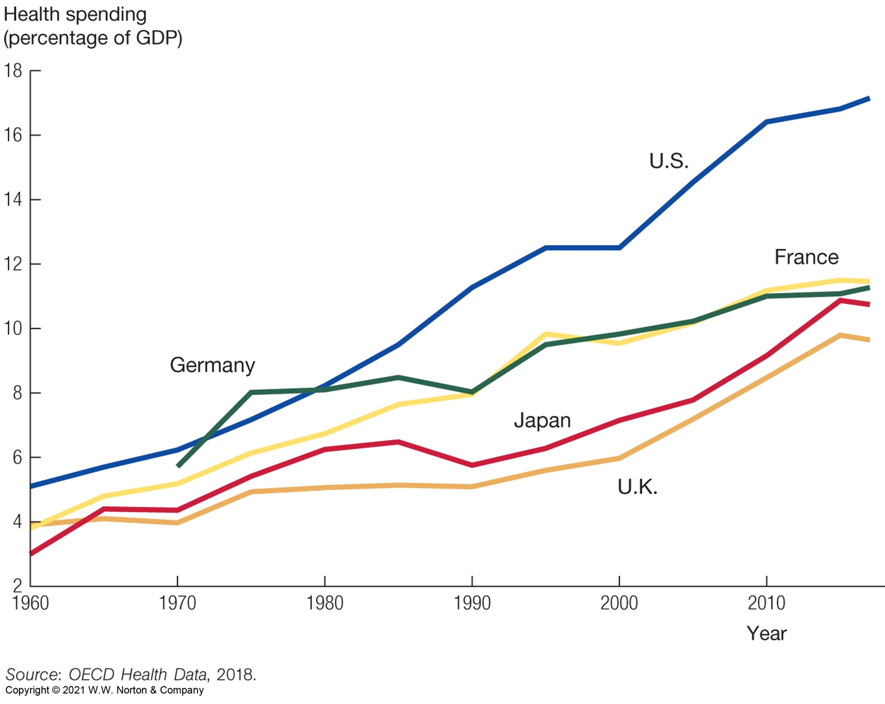
\includegraphics[width=0.5\linewidth]{Figures/fig_16_10}
	\end{figure}
	
\end{frame}

\begin{frame}[wide]{Possible Solutions?}
	\begin{itemize}
		\item Explanations for increasing health care costs:
		\vspace{3mm}
		\begin{itemize}
			\item Expensive medical technologies are raising expenditures
			\vspace{3mm}
			\begin{itemize}
				\item New technology is expensive although they are valuable
			\end{itemize}
			\vspace{3mm}
			\item Waste and fraud in the health system probably does not explain increasing expenses
			\vspace{3mm}
			\begin{itemize}
				\item e.g., Medical staff may ask patients to conduct unnecessary tests or procedures
				\item Or lack of 	incentive to actually provide enough services (e.g., roster limit)
			\end{itemize}
		\end{itemize}
	\end{itemize}
\end{frame}

%\begin{frame}[wide]{Possible Solutions?}
%	\begin{itemize}
%		\item A better alternative story: 
%		\begin{itemize}
%			\item Consumption is subject to diminishing returns
%			\begin{itemize}
%				\item As people grow richer over time, consumption rises, and the return to increasing consumption falls
%			\end{itemize}
%			\item Adding additional months of life is not subject to diminishing returns
%			\begin{itemize}
%				\item barely enough time to enjoy the riches already available to the upper/middle class
%			\end{itemize}
%			\item We may be shifting spending in typical consumption to health spending
%		\end{itemize}
%	\end{itemize}
%\end{frame}

\begin{frame}[wide]{Possible Solutions?}
	\begin{itemize}
		\item Possible solutions, other than raising taxes, include:
		\vspace{3mm}
		\begin{itemize}
			\item Private health insurance 
			\item Mandated savings in individual health-spending accounts
		\end{itemize}
		\vspace{6mm}
		\item These may create new problems of their own
		\vspace{3mm}
		\begin{itemize}
			\item Monopoly!?
			\item Scale effect!?
		\end{itemize}
	\end{itemize}
\end{frame}

%\begin{frame}[wide]{An Increase in the Investment Rate}
%	\begin{columns} 
%			% Column 1
%			\begin{column}{.5\textwidth}
%				\begin{itemize}
%					\item Suppose the investment rate increases permanently for exogenous reasons ($s'>s$)
%					\begin{itemize}
%						\item The investment curve rotates upward ($\bar{s}'\bar{A}  \bar{L}^{1-\alpha} K_t^\alpha > \bar{s}\bar{A}  \bar{L}^{1-\alpha} K_t^\alpha$)
%						\item The depreciation curve remains unchanged ($\delta K_t$)
%						\item The capital stock increases by transition dynamics to reach the new steady state
%						\begin{itemize}
%							\item This happens because investment exceeds depreciation ($sY_t>\delta K_t$)
%						\end{itemize}
%						\item The new steady state is located to the right
%					\end{itemize}
%				\end{itemize}
%			\end{column}
%			% Column 2    
%			\begin{column}{.5\textwidth}			
%				\begin{figure}
%					\centering
%					\includegraphics[width=1\linewidth]{"Figures/An Increase in the Investment Rate"}
%				\end{figure}
%			\end{column}%
%		\end{columns}
%\end{frame}

%\begin{frame}[wide]{Measuring the State of the Economy}
%	\begin{columns} 
%		% Column 1
%		\begin{column}{.5\textwidth}
%			\begin{table}[htbp]
%				\centering
%				\begin{tabular}{lrrrr}
%					& 2005  & 2006  & 2007  & 2008 \\
%					\hline
%					GDP   & 12.6  & 13.4  & 14.0    & 14.3 \\
%					(in trillions of \$) &       &       &       &  \\
%					Growth rate GDP &       & 0.063 & 0.045 & 0.021 \\
%					\hline
%				\end{tabular}%
%				\label{tab:addlabel}%
%			\end{table}%
%		\end{column}
%		% Column 2    
%		\begin{column}{.5\textwidth}			
%			
%			
%		\end{column}%
%	\end{columns}
%\end{frame}

\begin{frame}[wide]{Next Lecture}
	\begin{itemize}
		\item ...
	\end{itemize}
\end{frame}

\end{document}